\documentclass[paper=letter,11pt]{scrartcl}

\KOMAoptions{headinclude=true, footinclude=false}
\KOMAoptions{DIV=14, BCOR=5mm}
\KOMAoptions{numbers=noendperiod}
\KOMAoptions{parskip=half}
\addtokomafont{disposition}{\rmfamily}
\addtokomafont{part}{\LARGE}
\addtokomafont{descriptionlabel}{\rmfamily}
%\setkomafont{pageheadfoot}{\normalsize\sffamily}
\setkomafont{pagehead}{\normalsize\rmfamily}
%\setkomafont{publishers}{\normalsize\rmfamily}
\setkomafont{caption}{\normalfont\small}
\setcapindent{0pt}
\deffootnote[1em]{1em}{1em}{\textsuperscript{\thefootnotemark}\ }


\usepackage{amsmath}
\usepackage[varg]{txfonts}
\usepackage[T1]{fontenc}
\usepackage{graphicx}
\usepackage{xcolor}
\usepackage[american]{babel}
% hyperref is needed in many places, so include it here
\usepackage{hyperref}

\usepackage{xspace}
\usepackage{multirow}
\usepackage{float}


\usepackage{braket}
\usepackage{bbm}
\usepackage{relsize}
\usepackage{tcolorbox}

\def\ketY{\ensuremath{\ket {\Psi}}}
\def\iGeV{\ensuremath{\textrm{GeV}^{-1}}}
%\def\mp{\ensuremath{m_{\textrm{proton}}}}
\def\rp{\ensuremath{r_{\textrm{proton}}}}
\def\me{\ensuremath{m_{\textrm{electron}}}}
\def\aG{\ensuremath{\alpha_G}}
\def\rAtom{\ensuremath{r_{\textrm{atom}}}}
\def\rNucl{\ensuremath{r_{\textrm{nucleus}}}}
\def\GN{\ensuremath{\textrm{G}_\textrm{N}}}
\def\ketX{\ensuremath{\ket{\vec{x}}}}
\def\ve{\ensuremath{\vec{\epsilon}}}


\def\ABCDMatrix{\ensuremath{\begin{pmatrix} A &  B  \\ C  & D \end{pmatrix}}}
\def\xyprime{\ensuremath{\begin{pmatrix} x' \\ y' \end{pmatrix}}}
\def\xyprimeT{\ensuremath{\begin{pmatrix} x' &  y' \end{pmatrix}}}
\def\xy{\ensuremath{\begin{pmatrix} x \\ y \end{pmatrix}}}
\def\xyT{\ensuremath{\begin{pmatrix} x & y \end{pmatrix}}}

\def\IMatrix{\ensuremath{\begin{pmatrix} 0 &  1  \\ -1  & 0 \end{pmatrix}}}
\def\IBoostMatrix{\ensuremath{\begin{pmatrix} 0 &  1  \\ 1  & 0 \end{pmatrix}}}
\def\JThree{\ensuremath{\begin{pmatrix}    0 & -i & 0  \\ i & 0  & 0 \\ 0 & 0 & 0 \end{pmatrix}}} 
\def\JTwo{\ensuremath{\begin{bmatrix}    0 & 0 & -i  \\ 0 & 0  & 0 \\ i & 0 & 0 \end{bmatrix}}}
\def\JOne{\ensuremath{\begin{bmatrix}    0 & 0 & 0  \\ 0 & 0  & -i \\ 0 & i & 0 \end{bmatrix}}}
\def\etamn{\ensuremath{\eta_{\mu\nu}}}
\def\Lmn{\ensuremath{\Lambda^\mu_\nu}}
\def\dmn{\ensuremath{\delta^\mu_\nu}}
\def\wmn{\ensuremath{\omega^\mu_\nu}}
\def\be{\begin{equation*}}
\def\ee{\end{equation*}}
\def\bea{\begin{eqnarray*}}
\def\eea{\end{eqnarray*}}
\def\bi{\begin{itemize}}
\def\ei{\end{itemize}}
\def\fmn{\ensuremath{F_{\mu\nu}}}
\def\fMN{\ensuremath{F^{\mu\nu}}}
\def\bc{\begin{center}}
\def\ec{\end{center}}
\def\nus{$\nu$s}

\def\adagger{\ensuremath{a_{p\sigma}^\dagger}}
\def\lineacross{\noindent\rule{\textwidth}{1pt}}

\newcommand{\multiline}[1] {
\begin{tabular} {|l}
#1
\end{tabular}
}

\newcommand{\multilineNoLine}[1] {
\begin{tabular} {l}
#1
\end{tabular}
}



\newcommand{\lineTwo}[2] {
\begin{tabular} {|l}
#1 \\
#2
\end{tabular}
}

\newcommand{\rmt}[1] {
\textrm{#1}
}


%
% Units
%
\def\m{\ensuremath{\rmt{m}}}
\def\GeV{\ensuremath{\rmt{GeV}}}
\def\pt{\ensuremath{p_\rmt{T}}}


\def\parity{\ensuremath{\mathcal{P}}}

\usepackage{cancel}
\usepackage{ mathrsfs }
\def\bigL{\ensuremath{\mathscr{L}}}

\usepackage{ dsfont }



\usepackage{fancyhdr}
\fancyhf{}

%\documentclass[margin,line]{res}
\usepackage{braket}
\usepackage{bbm}
\usepackage{relsize}

\def\ketY{\ensuremath{\ket {\Psi}}}
\def\iGeV{\ensuremath{\textrm{GeV}^{-1}}}


\def\ABCDMatrix{\ensuremath{\begin{pmatrix} A &  B  \\ C  & D \end{pmatrix}}}
\def\xyprime{\ensuremath{\begin{pmatrix} x' \\ y' \end{pmatrix}}}
\def\xyprimeT{\ensuremath{\begin{pmatrix} x' &  y' \end{pmatrix}}}
\def\xy{\ensuremath{\begin{pmatrix} x \\ y \end{pmatrix}}}
\def\xyT{\ensuremath{\begin{pmatrix} x & y \end{pmatrix}}}

\def\IMatrix{\ensuremath{\begin{pmatrix} 0 &  1  \\ -1  & 0 \end{pmatrix}}}
\def\IBoostMatrix{\ensuremath{\begin{pmatrix} 0 &  1  \\ 1  & 0 \end{pmatrix}}}
\def\JThree{\ensuremath{\begin{pmatrix}    0 & -i & 0  \\ i & 0  & 0 \\ 0 & 0 & 0 \end{pmatrix}}} 
\def\JTwo{\ensuremath{\begin{bmatrix}    0 & 0 & -i  \\ 0 & 0  & 0 \\ i & 0 & 0 \end{bmatrix}}}
\def\JOne{\ensuremath{\begin{bmatrix}    0 & 0 & 0  \\ 0 & 0  & -i \\ 0 & i & 0 \end{bmatrix}}}
\def\etamn{\ensuremath{\eta_{\mu\nu}}}
\def\Lmn{\ensuremath{\Lambda^\mu_\nu}}
\def\dmn{\ensuremath{\delta^\mu_\nu}}
\def\wmn{\ensuremath{\omega^\mu_\nu}}
\def\be{\begin{equation*}}
\def\ee{\end{equation*}}
\def\bc{\begin{center}}
\def\ec{\end{center}}
\def\nus{$\nu$s}
%\def\xMu{\ensuremath{x^\mu}

\usepackage{fancyhdr}

\fancyhf{}
\lhead{\Large 33-444} % \hfill Introduction to Particle Physics \hfill Spring 2020}
\chead{\Large Introduction to Particle Physics} % \hfill Spring 2020}
\rhead{\Large Spring 2020} % \hfill Introduction to Particle Physics \hfill Spring 2020}

\begin{document}
\thispagestyle{fancy}

\begin{center}
{\huge \textbf{Lecture 33}}
\end{center}

{\fontsize{14}{16}\selectfont

\textbf{\underline{Neutrino Physics}} 

OK so we left off in

\textbf{- 1934:} Where we get Fermi's theory of the weak interactions.  We have already talked in this course about how much of a big deal this was. 
It was Bold and did things that no other theory before had done. 

Model: 

\bc
$n \rightarrow p + e + \nu$
\ec

First time we have physics interaction that can change the particle type. 

But most importantly it allows calculations 

eg: if this is how \nus\ are produced, then you can calculate how to detect this particle. 

\bc
$\nu + p \rightarrow e + n$
\ec

and it turns out that this has non-zero cross-section. 

You can actually calculate the cross-section and it turns out to be ridiculously small.

So this made it clear why \nus\ hadn't yet been seen, but it also put damper on hopes of finding them. 



Change gears a bit ... Nothing happens w/\nus\ for 20 years.

\noindent\rule{\textwidth}{1pt}

However meanwhile, 

\textbf{- 1935:} Yukawa is thinking about how ns and ps interact in the nucleus and predicts that there is a new particle he calls a ``Meson'' responsible. 
Estimates the mass of the Meson $\sim 100$ MeV


\textbf{- 1936:} One of the amazing things that sometimes happens in history, people studying cosmic rays found a meson with m = 106 MeV. (very impressive!)
However this turns out to be wrong and this lead to a period of mass confusion.   
In particular, if produced in a cosmic ray there is no way that the particle predicted by Yukawa can make to the your detector on earth. 
This took a long time to sort out

\textbf{- 1947:} Get the ``2 Meson  hypothesis'' that there are really 2 particles the ``$\mu$-meson'' (or today $\mu$) and the ``$\pi$-meson'' (today pion) 
A little later the $\pi$ was discovered, this time by doing cosmic ray experiments really high up in the mountains. (Pyrenees I believe?)

Now know that the pion decays to a muon:

\bc
$\pi^- \rightarrow \mu^- + \nu$
\ec

\noindent\rule{\textwidth}{1pt}

\textbf{Now in 1950s:} 
\nus\ start to become interesting again. 
Of course, its not b/c the cross section changed, but b/c people invented Atomic Bombs for the war...

Turns out that A-Bombs are ridiculous sources of \nus. 
Fluxes you could get out of an atomic bomb was incredibly large. 
$\Rightarrow$ could hope to make up for the really tiny $\sigma$ w/really big flux. 

\clearpage

\textbf{1956s: - $\nu$ is discovered}  (Reines-Cowan) 

Here is an actual experiment that was proposed: 

\begin{figure}[h!]
\centering
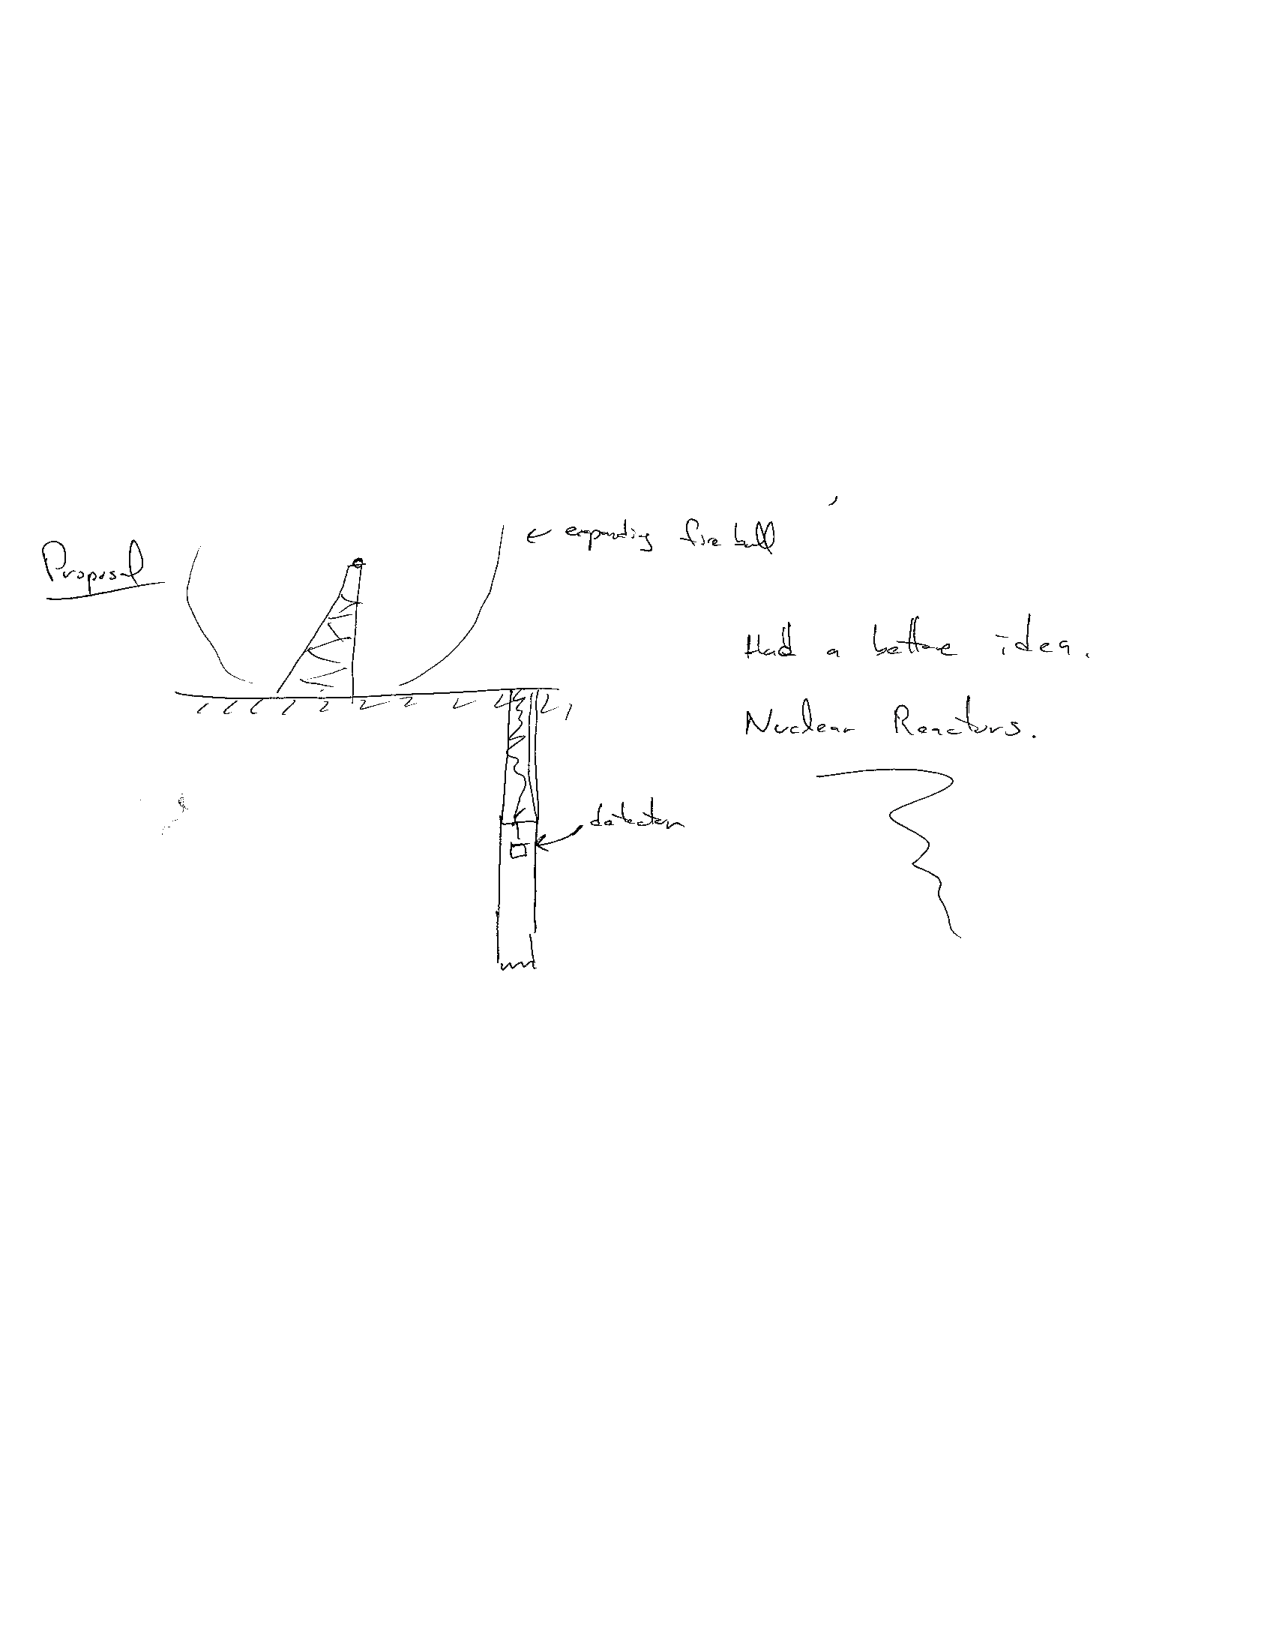
\includegraphics[width=1.0\textwidth]{./ABomb.pdf}
\end{figure}



Drop your detector when the bomb goes off. 
(Don't want it touching the earth b/c all hell is breaking loose from the explosion.)
Make recordings as its falling. 

Unfortunately, did not try this experiment....
Had a better idea instead: use nuclear reactors, which are also impressive sources of \nus.

\clearpage 

OK so we want to measure:
n
\be
\bar{\nu}_e + p \rightarrow e^+ + n
\ee

1) Need to see this positron 2) need a lot of mass b/c the cross section is small. 

Turns out that you don't see the positron directly. 
It wonders around and annihilates with an electron $e^+e^-\rightarrow \gamma\gamma$; what you see are the photons. 

Now there is actually a lot of stuff that looks like $e^+e^-\rightarrow \gamma\gamma$ in these massive detectors.
So its hard to convince yourself that you are actually seeing the \nus.
But if you pick the right nucleus for the stuff your detector is made of you can also see the neutron. 
(Very clever idea) You can get the reaction:
\be
n+N \rightarrow N^* \rightarrow N + \gamma
\ee
which turns out (for complicated nuclear physics reasons) has a well-defined time scale associated to it. 

So the way you can really convince yourself you are seeing \nus\ is by looking for a $e^+e^-\rightarrow \gamma\gamma$ signal followed after by the photon form the $N^*$ after a very specific time window. 
This ``coincidence'' of signals allows you to tease out the \nus\ form the other backgrounds.

This is how \nus\ where discovered for the first time and actually we still use this same technique today.

\noindent\rule{\textwidth}{1pt}

\textbf{\underline{Back to $\mu$'s for a moment}}

As we talked about before $\mu$'s look a lot like a heavy electron. 
People have been thinking a lot about how muons fit into the theory for a long time. 
We still don't know the answer.  
Famous quote from this period I.I. Rabi. ``Who ordered that?''

One very obvious idea is that muons are excited electrons. (Behave like electrons with more energy or more mass) 

However if muons are excited electrons then you would expect to see:
\be
\mu^- \rightarrow e^- \gamma
\ee
We looked for this and didn't see it. 

In the mean time people figured out that muons decay via the weak interaction: 
\be
\mu^- \rightarrow e^- + \nu + \bar{\nu}
\ee
(...Has to be two \nus\ for same reason you need a $\nu$ to explain $\beta$ decay) 

\begin{figure}[h!]
\centering
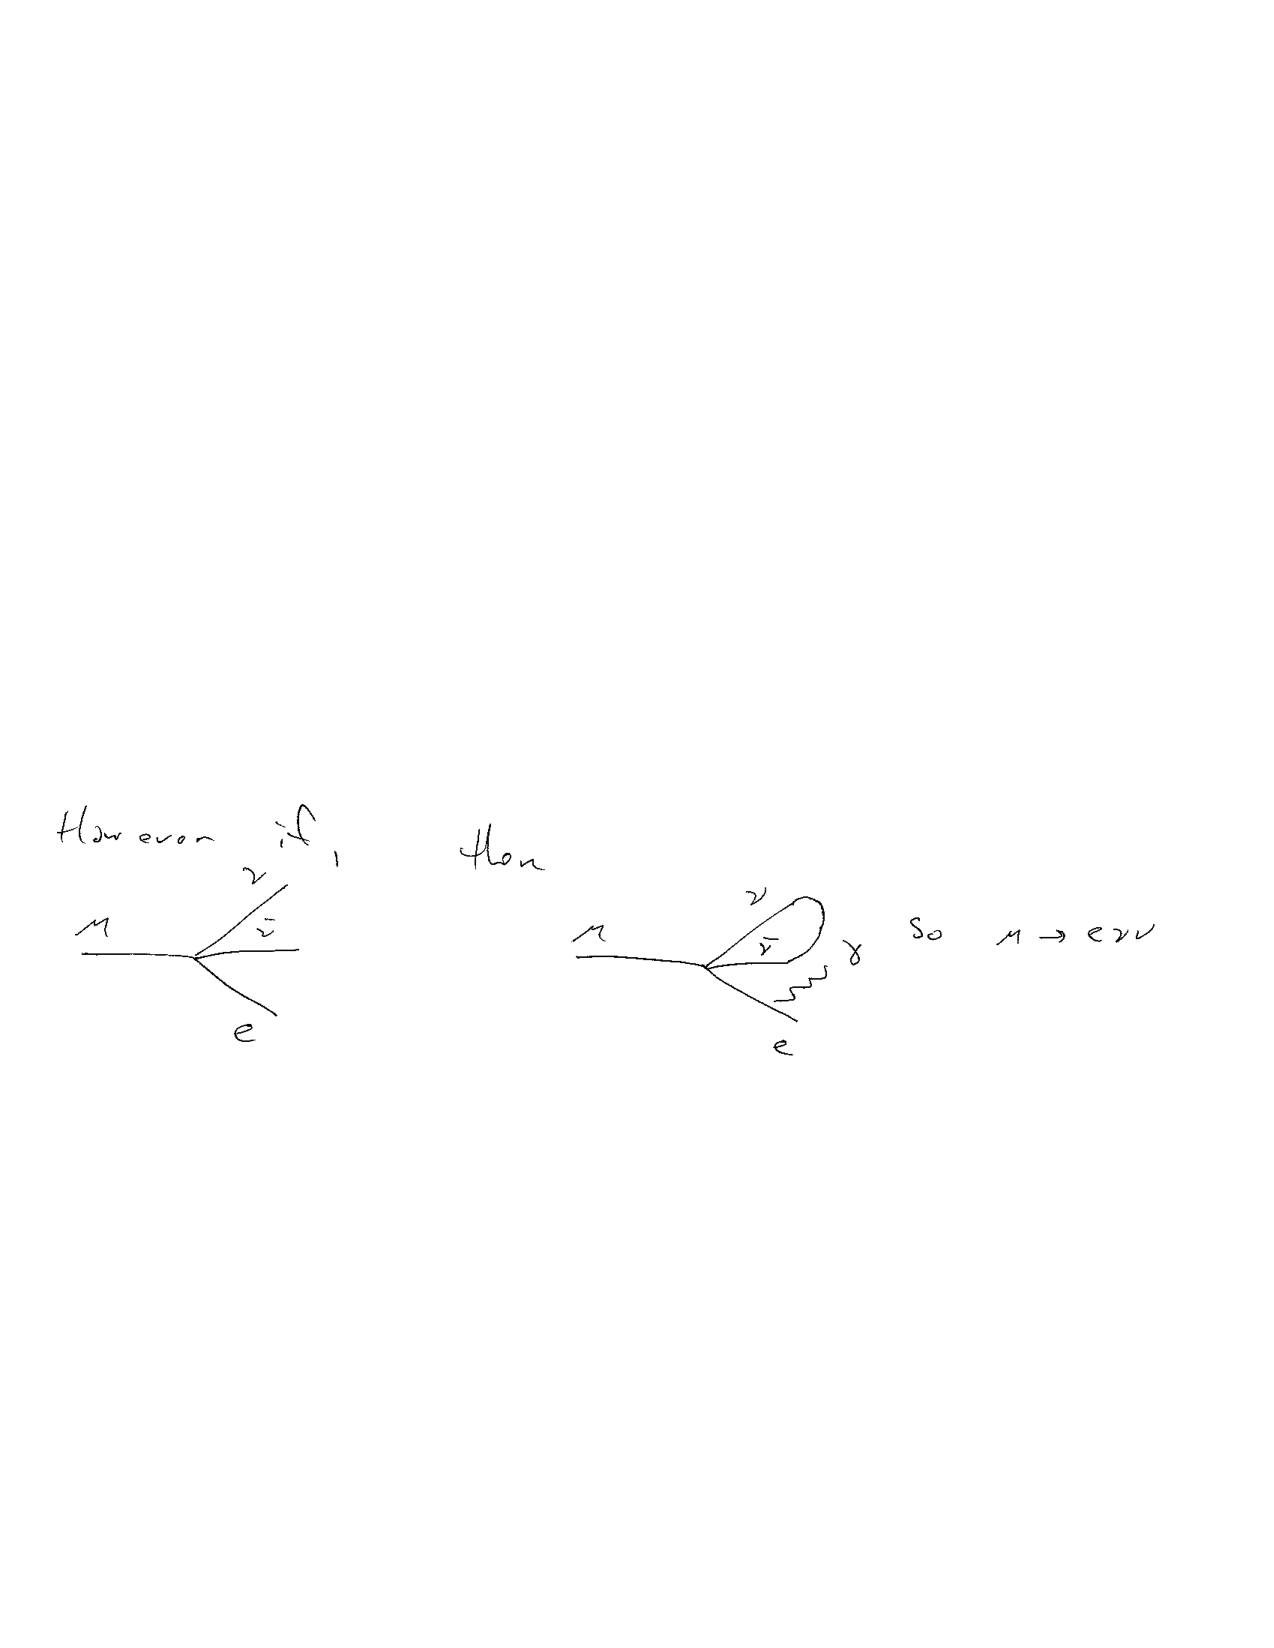
\includegraphics[width=1.0\textwidth]{./MuToEg.pdf}
\end{figure}

And you can also calculate the rate you expect for this reaction. 

Turns out $Br(\mu\rightarrow e \gamma) \sim 10^{-4}$ but we had measured that $Br(\mu\rightarrow e \gamma) < 10^{-7}$.
So we had a big problem. 

Solution to this was the ``2 neutrino hypothesis''. 
Ideas is that if the neutrinos produced are different, this would prevent you from closing the loop. 
Another way to say this is that there must be a conserved quantity ``Lepton flavour Number''. 
Such that this quantum number is conserved in these reactions.  
So really whats happening is:
\be
\mu^- \rightarrow e^- + \nu_e + \bar{\nu}_\mu
\ee

But how can we confirm that this is what is really going on?... $\nu$-Beams.

\noindent\rule{\textwidth}{1pt}

\textbf{\underline{$\nu$-beams} }

Major development in the field.

We talked about why pions decay mainly to muons and not electrons. 
If you believe in muon-number conservation you expect
\be 
\pi \rightarrow \mu^+ \nu_\mu
\ee 

If you then make the \nus\ you get from this decay hit something you would expect to see

\be
\nu_\mu + X \rightarrow \mu^- + Y
\ee
and not see
\be
\nu_\mu + X \rightarrow e^- + Y
\ee

This is very nice because it is kinetically easier to produce electrons than muons. 
So if these \nus\ can do both, you would expect to see more electrons if anything. 

And the way you produce a beam of $\nu_\mu$s is as follows:

\begin{figure}[h!]
\centering
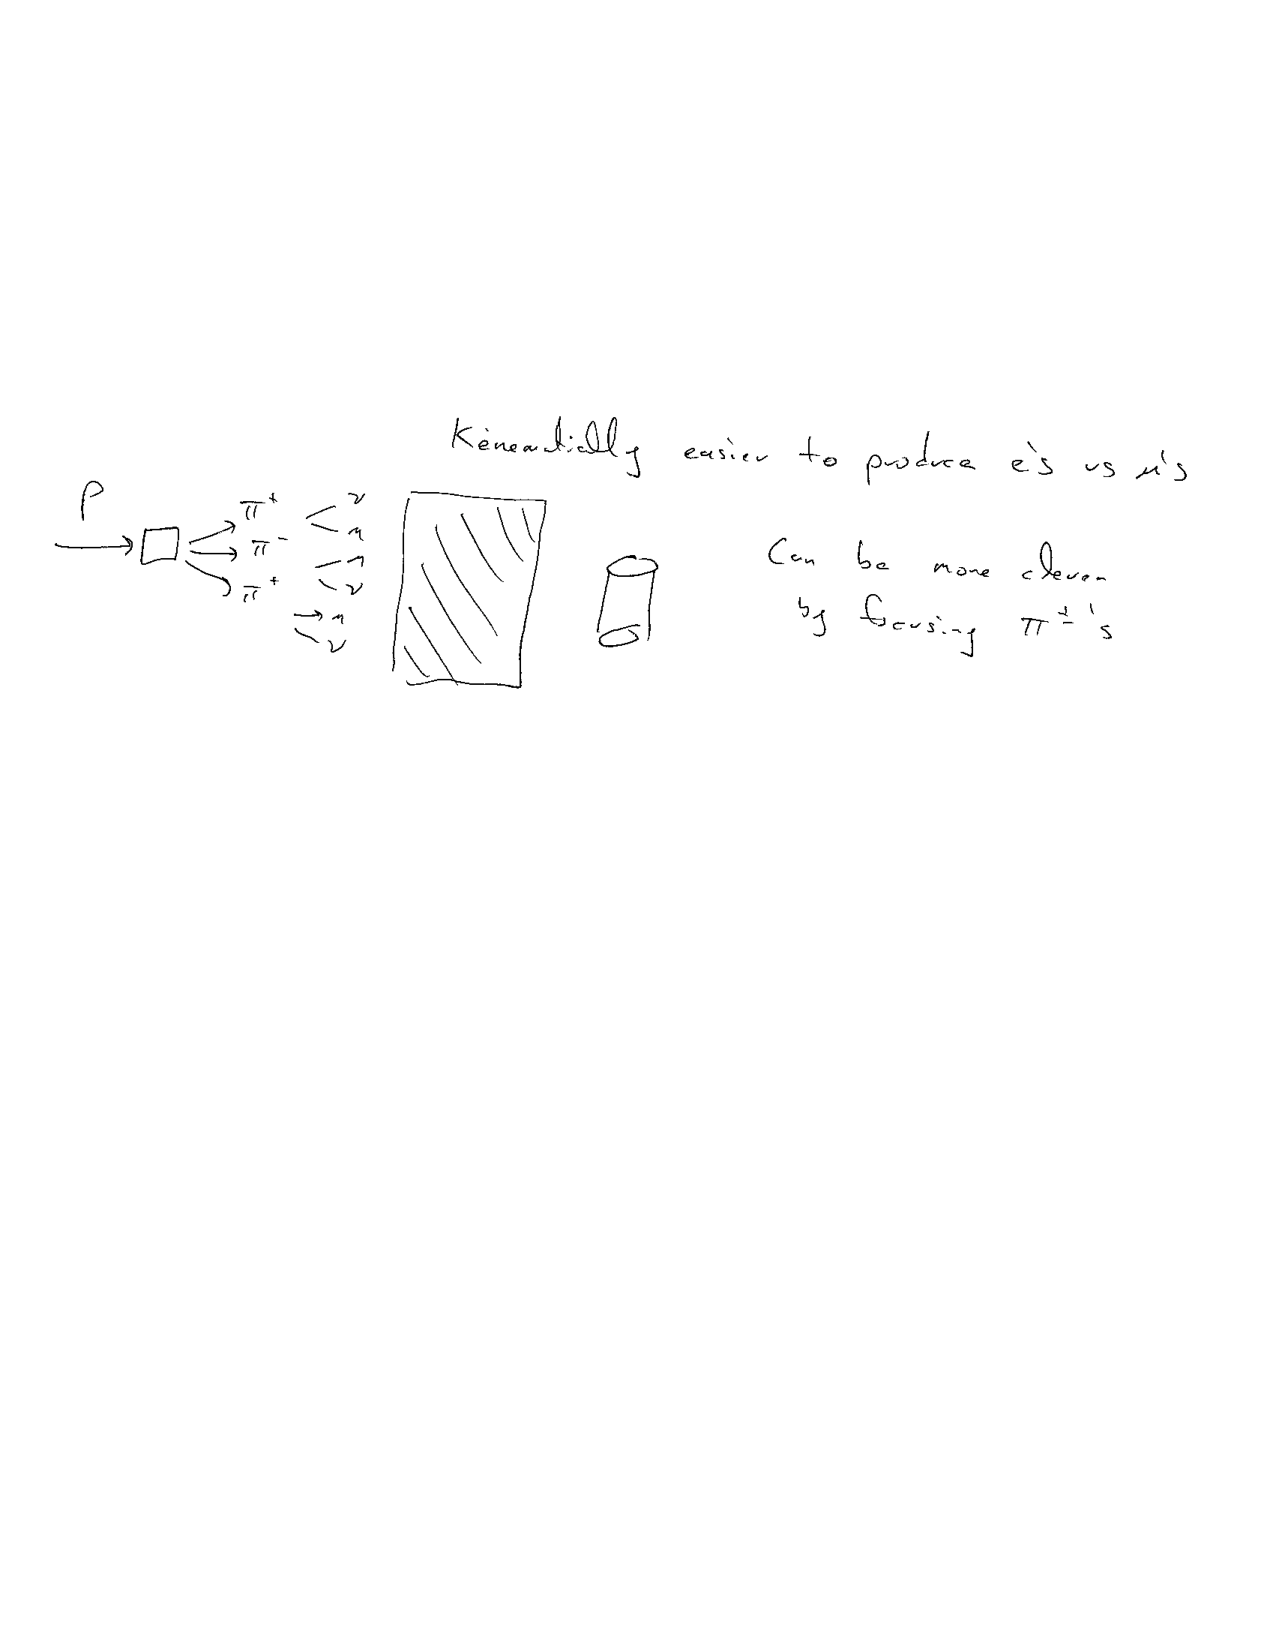
\includegraphics[width=1.0\textwidth]{./NuBeam.pdf}
\end{figure}

The only thing that can make it through the shielding (usually a big pile of dirt or lead) is the \nus.

\textbf{- 1962:} Discovery of $\nu_\mu$

\textbf{- 1970s:} Discovered $\tau$, People said there has to be a $\nu_\tau$ as well. 

\textbf{- 1980s:} Remember LEP found $N_\nu$ = 3 with very small uncertainty.  
Can think of this as confirmation of the tau neutrino.  
However you really want to see direct evidence for $\nu_\tau$, eg: you want to see tau neutrino scattering off of something. 
This turns out to be ridiculously hard! 

Did not have direct evidence of $\nu_\tau$ hitting something \textbf{\underline{until 2001}}


The way you see this is with

\be
\nu_\tau + X \rightarrow \tau + Y 
\ee

This is hard for many reasons:
\begin{itemize}
\item[-] $\tau$s are heavy, need high-energy $\nu_\tau$s
\item[-] How do you get $\nu_\tau$s ? Need B's (and D's) but hard to produce these. 
\item[-] Bs (Ds) decay mainly to $\tau$s for same reason that $\pi$s decay mainly to muons, however b/c the mass is big also get a lot of $\nu_\mu$s
\item[-] How do you see a  $\tau$ ? Can see $\tau \rightarrow \mu$. The muon is ``easy'' to see. But you have a lot of $\nu_\mu$s. So you really need to see the $\tau$ move before decaying.
\item[-] Unfortunately the $\tau$ has a very short lifetime, so you need very good position resolution to see evidence for it moving. 
\item[-] Of course all this is happening in a very dense environment (b/c the cross sections are so small) 
\end{itemize}

The DUoNUT collaboration directly observed the $\nu_\tau$ interactions in 2001. 
You should look up details online. 

For scale, we have seen way more Higgs bosons than $\nu_\tau$s

\noindent\rule{\textwidth}{1pt}

\textbf{OK end of historical introduction} Brief recap

So we knew about three neutrinos. 
\begin{center}
$\nu_e + X  \rightarrow e + Y $

$\nu_\mu + X \rightarrow \mu + Y $

$\nu_\tau + X  \rightarrow \tau + Y$
\end{center}

These are named b/c the $\nu_e$ gives you a e the $\nu_\mu$ give you a $\mu$ and so on. 

And we had global symmetries associated to all this. 
Can assign quantum numbers in such away that you have a  conserved electron number, muon number, and tau number.

\noindent\rule{\textwidth}{1pt}

\underline{\textbf{\nus\ are interesting particles in the SM. }}

No color/ No charge / only talk to W,Z  (ie: only weak interactions) 
This of course makes them incredibly hard to study, but we have nonetheless we have made lots of progress doing neutrino experiments. 

Doing $\nu$ experiments was a huge deal already in the 70s, not so much b/c people cared about \nus. 
Main reason for this is that they were a great way of studying the weak interaction. 
If you use electrons you have EM as ``Background''. 
EM interactions get in the way. 

Other more technical things, (at least until recently) \nus\ supposed to have no mass. 
This fact came from a combination of things. 
1) no observation of an effect of the neutrino mass. 
2) \nus\ only have the weak interactions: purely left-handed (Talked about this when talked about Higgs)

\textit{Over the last 20 years we have become convinced that this is wrong. }

We now have evidence that it is possible to produce a muon neutrino, let it propagate a long distance and produce a tau. 
(or take an electron neutrino and have it produce a muon. )

Turns out only happens if you wait long enough. 

What we now know is that \nus\ ``Flavour change'' as a function of how far the \nus\ travel (Baseline)
This is a really big deal. 

We will talk about how we got there now...This will now be less historical. 

\noindent\rule{\textwidth}{1pt}

\underline{\textbf{Solar \nus}}

Very old problem that started out in the 60s. 

First thing that happened was that people started to understand solar \nus.\

This is a really exciting very important topic that also started in the 30s and 40s, or even way before when people tried to understand how the sun works.
Were puzzled by the fact that the sun was emitting a ridiculous amount of energy and they didnt know where it was coming from. 

Its a puzzle. 
The sun is radiating like mad... and somehow it keeps on doing that and if you've never thought about this its pretty weird. 
Its been doing it for billions of years and people had absolutely no idea how this works.  
Subtle effect that requires microscopic physics.  
Nuclear fusion process that relies on the fact that you can change your mass a little bit and convert that into a ridiculous amount of energy.
Which is how the sun works. 
Took a long time to get this right in the details. 


\underline{Bottom line}: Solar fusion takes lighter nuclei and might bigger ones.
Also important to know is that the sun is very proton rich, not many neutrons (lots of electrons), so in the process of forming nuclei you can convince yourself that you also need to emit a lot of \nus. 
not anti-\nus, proper \nus.   
This is the opposite of $\beta$ decay. 

$\beta$ decay is usually from nuclei that have too many neutrons in them. 
So they are happy to convert into protons and emit anti-neutrinos at the same time. 
On the flip side if you have an environment that is proton-rich and you are creating nuclei that means you are converting protons into neutrons; to balance out the charge you have to spit out positrons and therefore neutrinos to conserve lepton number. 
So the sun is a very efficient machine for producing neutrinos. 

When people finally figured out how the sun worked they said ``hey look the sun is spitting out all these \nus\ wouldn't it be great if we could see them.''
People started thinking about how to do this. 

We can calculate the flux of neutrinos coming from the sun,  its a very high number. $10^{11}/s/cm^2$ on earth. 
And we can calculate what energies they have.  
Heres what you get:

\begin{figure}[h!]
\centering
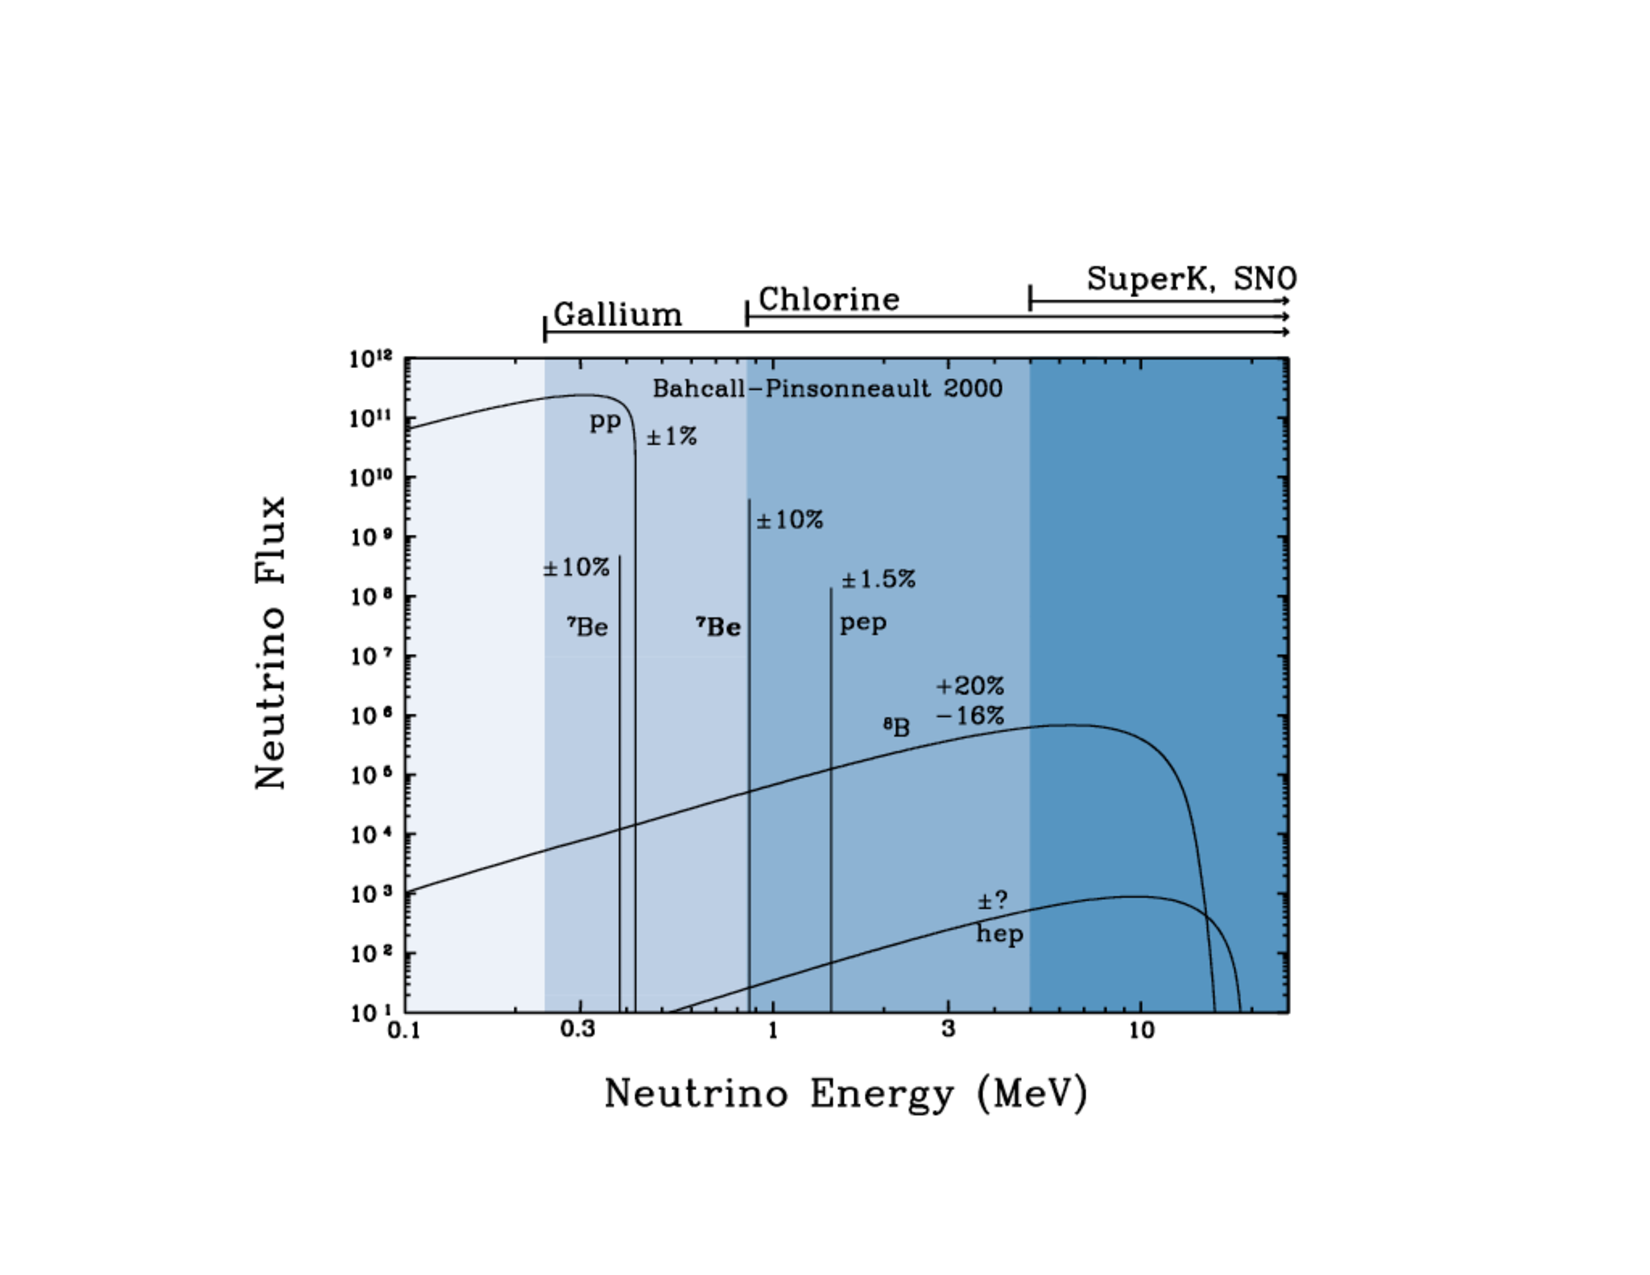
\includegraphics[width=1.0\textwidth]{./NuFromSun.pdf}
\end{figure}

Will pick up here next time...



}
\end{document}


